\documentclass[12pt]{article}
\providecommand{\normalsfcodes}{}

\usepackage{sbc-template}
\usepackage{graphicx,url}
\usepackage[utf8]{inputenc}
\usepackage[T1]{fontenc}
\usepackage[english]{babel}
\makeatletter\providecommand{\bbl@normalsf}{}\makeatother
\usepackage{amsmath,amssymb}
\usepackage{booktabs}
\usepackage{multirow}
\usepackage{array}
\usepackage{float}
\usepackage[authoryear,round]{natbib}
% sbc-template redefines \@lbibitem at the end of the preamble, which breaks natbib's
% author-year labels; keep natbib's definition.
\makeatletter
\let\NATsaved@lbibitem\@lbibitem
\AtBeginDocument{\let\@lbibitem\NATsaved@lbibitem}
\makeatother
\usepackage[colorlinks=true,citecolor=blue,linkcolor=black,urlcolor=blue]{hyperref}

\graphicspath{{../figs/journal/}}

\sloppy

\renewcommand{\topfraction}{0.9}
\renewcommand{\bottomfraction}{0.8}
\renewcommand{\textfraction}{0.07}
\renewcommand{\floatpagefraction}{0.85}
\setcounter{topnumber}{3}
\setcounter{totalnumber}{5}

\newcommand{\SIB}{BA-TOS~[SIBGRAPI'26]}
\newcommand{\FIX}{BA-TOS + corrected flattening}
\newcommand{\SF}{BA-TOS-SF}
\newcommand{\CP}{Cellpose-SAM}
\newcommand{\rg}{r_{\mathrm{granulo}}}

\title{BA-TOS-SF: Scale-Free Boundary-Aware Tree-of-Shapes Segmentation of Grains in 3D Micro-CT, with External Validation and Foundation-Model Benchmarking}

\author{Felipe Vilhena Dias\inst{1}, Silvio Jamil Ferzoli Guimarães\inst{1},\\ Yukiko Kenmochi\inst{2}, Nicolas Passat\inst{3},\\ Zenilton Kleber Gonçalves do Patrocínio Júnior\inst{1}}

\address{Laboratory of Image and Multimedia Data Science (IMScience),\\
Pontifícia Universidade Católica de Minas Gerais (PUC Minas),\\ Belo Horizonte, MG, Brazil
\nextinstitute
GREYC, UMR CNRS 6072, Université de Caen Normandie, Caen, France
\nextinstitute
CReSTIC, Université de Reims Champagne-Ardenne, Reims, France}

\begin{document}

\maketitle

\begin{abstract}
This undergraduate research project consolidates and improves BA-TOS, a training-free method for 3D grain
instance segmentation in micro-computed tomography (micro-CT) that selects watershed markers from a Tree of
Shapes (ToS). The published method had three open points: a failure on two crops that contain the specimen
boundary, a large number of hand-set constants, and an evaluation on a single specimen. We show that the
boundary failure is caused by exterior air biasing an intensity offset, and that a one-line, specimen-only
offset removes it (development crop-macro F1@0.50 from 0.824 to 0.976). We then propose BA-TOS-SF, a scale-free
version in which a granulometric (pattern-spectrum) estimate sets every size constant and all thresholds are
computed on the specimen only; 43 fixed voxel-size constants and 9 ad-hoc thresholds or grey-level guards are
removed. On a held-out set of 52 crops from six specimens, defined by a GT-free rule committed before cutting,
BA-TOS-SF reaches crop-macro F1@0.50 of 0.912, against 0.538 for the published method. A one-at-a-time audit of 96
constants identifies 25 influential ones. Finally, BA-TOS-SF is benchmarked against the Cellpose-SAM foundation
model, which, used with default settings, reaches 0.998 on the same held-out crops. The remaining gap is traced to
a single mechanism, the ToS candidate capacity on large grains.
\end{abstract}

% ---------------------------------------------------------------------------
\section{Introduction}

X-ray micro-computed tomography (micro-CT) enables non-destructive three-dimensional observation of the internal
structure of materials at particle scale. In granular materials, this capability supports quantitative studies of
particle morphology, orientation, contacts, rearrangement, and deformation. Tomography-based investigations have
shown that particle morphology strongly influences granular deformation processes, making reliable identification
of individual grains a prerequisite for subsequent quantitative analysis \citep{pinzon2025}. Because morphological
measurements are computed from the segmented support of each particle, segmentation errors propagate directly to
estimates of volume, surface area, equivalent diameter, orientation, and contact geometry.

Transforming a micro-CT volume into a set of individualized particles remains challenging. Grains are densely
packed, frequently touch each other, may exhibit similar grey-level distributions, and are affected by
acquisition noise, partial-volume effects, and reconstruction artifacts. A conventional workflow separates
foreground from background, for instance with Otsu's criterion \citep{otsu1979}, and then applies a distance-based
or marker-controlled watershed to split touching particles \citep{beucher1979,soille2003}. The final partition
depends strongly on marker quality: excessive markers cause over-segmentation, whereas missing markers merge
distinct grains.

This TCC builds on our previous work, BA-TOS \citep{dias2026}. BA-TOS extracts dark candidate regions from a 3D
Tree of Shapes (ToS), rejects candidates connected to the crop boundary, refines them into internal markers, and
runs a marker-controlled distance watershed inside an Otsu mask. A GT-free safeguard replaces the ToS markers by
distance-transform markers when their supports collapse to a few voxels. On 12 crops of one specimen, BA-TOS
reached a crop-macro F1@0.50 of $0.906 \pm 0.210$ with the safeguard and $0.824 \pm 0.367$ without it. The
published method left three points open:
\begin{enumerate}
  \item \textbf{A failure on two boundary crops.} On the two crops containing the specimen membrane and exterior
        air, the ToS supports collapsed (F1 0.012 without the safeguard). The safeguard limited the damage but the
        cause was not identified.
  \item \textbf{Many constants.} The pipeline has close to a hundred constants, many of them absolute sizes in
        voxels or absolute grey levels, and its sensitivity had been measured on a single crop only.
  \item \textbf{A single specimen.} The same 12 crops were used for design and evaluation, with no held-out or
        external data.
\end{enumerate}

The third checkpoint (PC3) of this TCC proposed to replace the marker-plus-watershed stage by a direct selection of
instances in the hierarchy. This alternative was explored: extinction-based selection of ToS minima (by volume,
dynamics, or their product, with and without uniqueness rules) reached at best F1@0.50 = 0.906 on the development
crop, against 0.985 for the BA-TOS selector, because secondary minima inside a grain split it into several
instances. It was therefore set aside in favour of strengthening the marker-based pipeline, which is the subject of
this report.

\textbf{Objectives.} The general objective is to turn BA-TOS into a method that is robust, independent of grain
scale, and validated on data not used for its design, and to position it against current foundation models. The
specific objectives are: (i) explain and correct the boundary-crop failure; (ii) replace absolute constants by
quantities derived from the image (BA-TOS-SF); (iii) audit the sensitivity of all constants on the development
crops; (iv) evaluate on a pre-registered held-out set of 52 crops from six specimens; (v) compare with Cellpose-SAM
under the same protocol, including robustness and boundary fidelity; and (vi) prepare the full-volume application,
grain tracking, and morphological analysis for TCC~II.

Figure~\ref{fig:slices} gives an overview of the four methods compared throughout: \SIB{} (the published method),
\FIX{} (the published method with the one-line offset correction of Section~\ref{sec:diag}), \SF{} (the proposed
scale-free method), and \CP{} (default settings).

\begin{figure}[t]
\centering
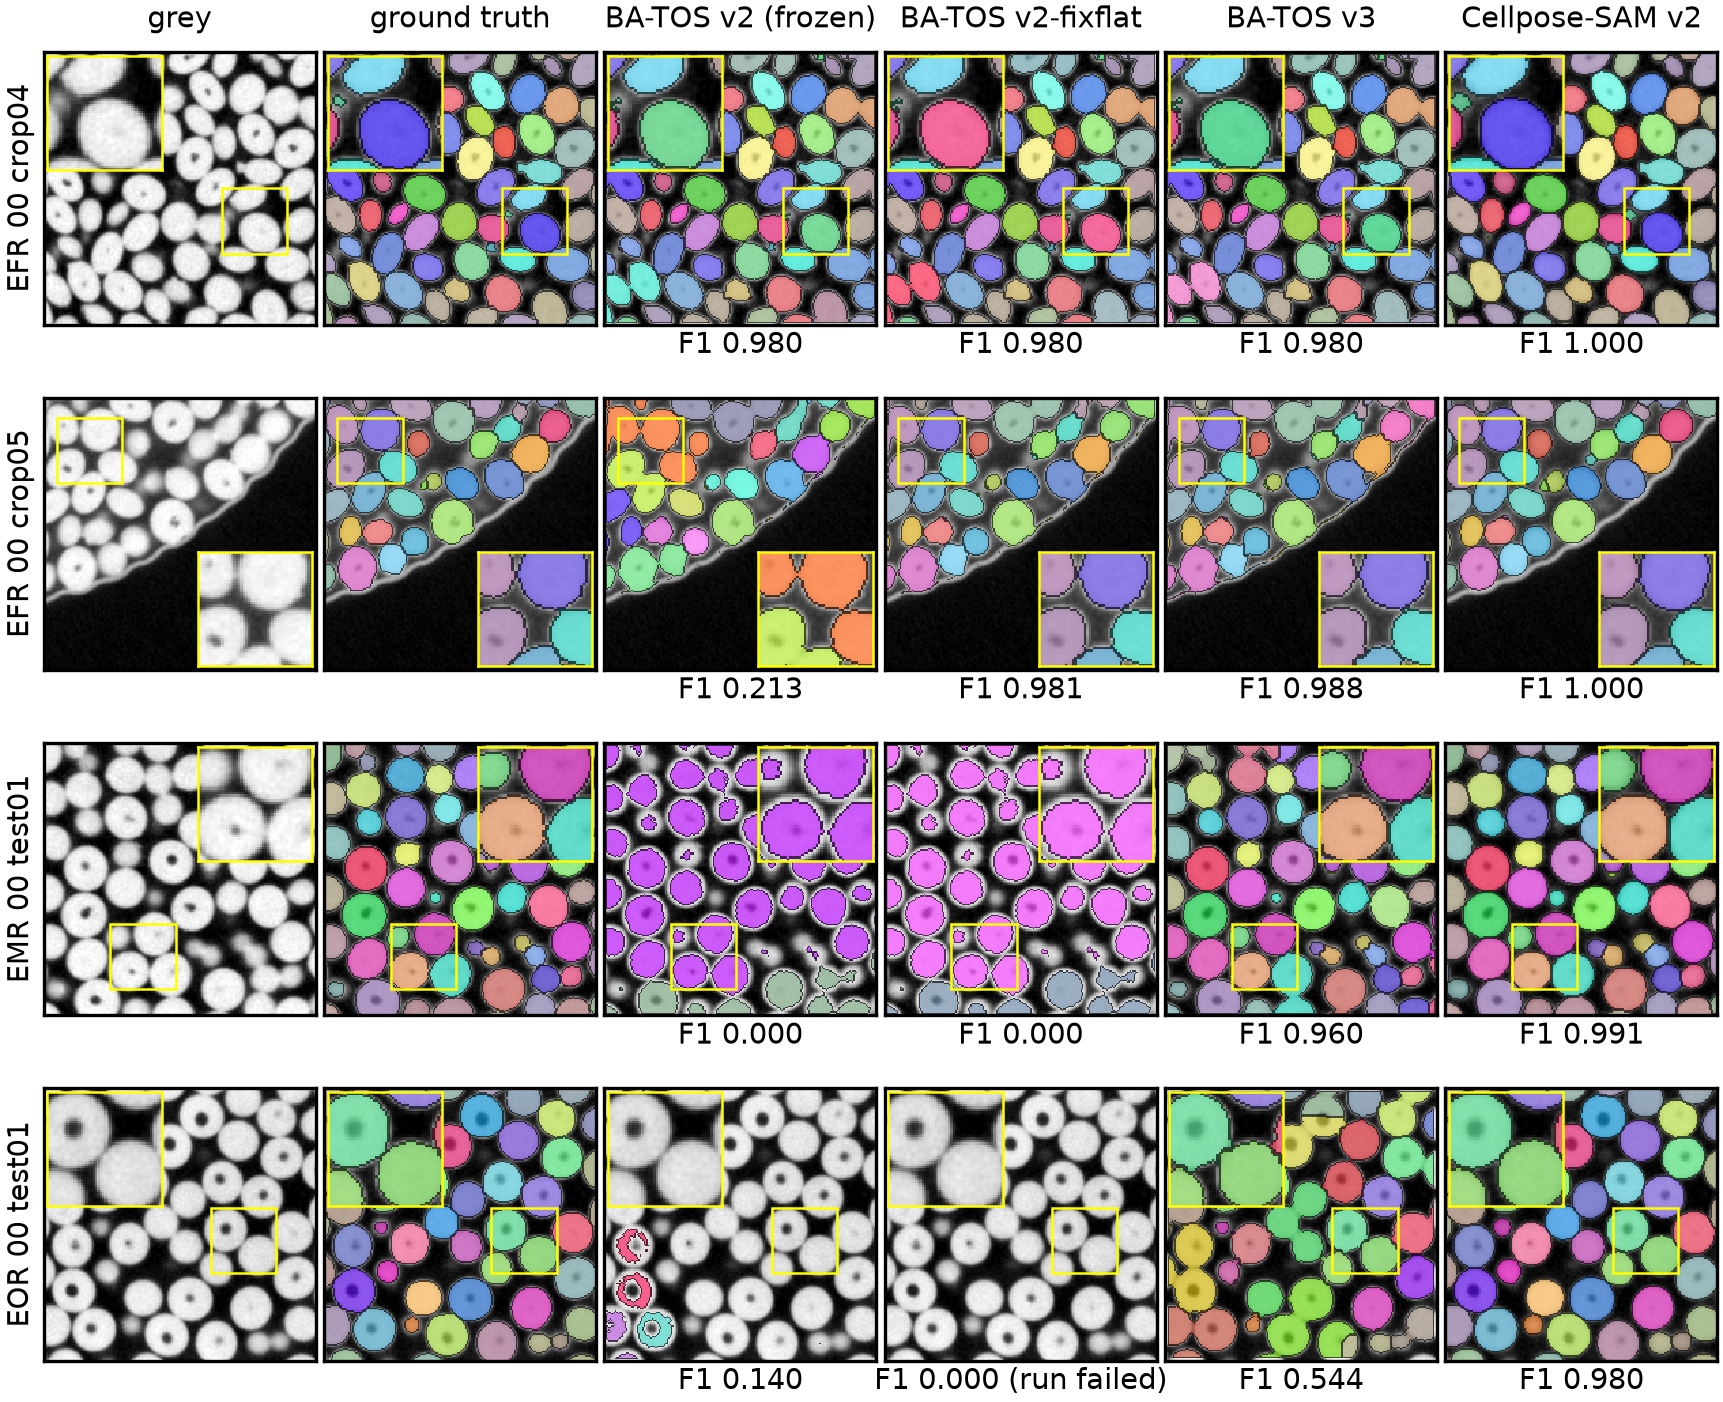
\includegraphics[width=\textwidth]{fig1_qualitative_slices.png}
\caption{Central $xy$ slice ($z=100$) of four $200^3$ crops (rows): the development crop EFRGP01\_00\_crop04, the
boundary crop EFRGP01\_00\_crop05 (membrane and exterior air), and interior test crops of specimens EMR and EOR.
Columns: grey value, ground truth, \SIB, \FIX, \SF, \CP. A prediction matched to a GT grain (3D IoU $>0.5$) takes
its colour; excluded GT is desaturated; insets magnify the yellow window. Under each panel: F1@0.50 of the whole
3D crop, no-marker evaluation, no size filter.}
\label{fig:slices}
\end{figure}

% ---------------------------------------------------------------------------
\section{Literature Review and Related Work}

\subsection{Particle separation and morphological analysis in micro-CT}

The literature on granular micro-CT commonly treats instance separation as an intermediate step required before
quantitative morphology can be trusted. The standard morphological route starts from a foreground mask and
separates touching objects with a distance transform and watershed \citep{beucher1979,soille2003}. This approach
is interpretable, training-free, and directly applicable to three-dimensional binary supports, but it transfers
much of the difficulty to seed or marker construction.

Several studies therefore concentrate on controlling watershed errors rather than replacing the watershed
itself. \citet{burgmann2022} use an adaptive $h$-extrema transform to suppress irrelevant extrema before watershed
and estimate parameters from packing characteristics. \citet{alshembari2024} begin with a watershed partition and
use a random forest to detect fragments that should be merged. \citet{wang2025} likewise retain watershed as an
initialization, automatically correct over-segmentation, and then refine grain boundaries through a level-set
formulation. These studies progressively improve robustness and boundary quality, but their common structure is
\emph{partition first, repair or refine afterward}, and the principal weaknesses remain marker multiplicity,
missing seeds, and inaccurate contact boundaries.

\subsection{Hierarchical mathematical morphology and the Tree of Shapes}

Hierarchical morphological representations organize regions according to inclusion, making it possible to reason
about objects at several intensity levels without independently processing each threshold. Component trees and
connected operators established that region-level filtering can simplify an image without creating new contours
\citep{salembier1998}. The Tree of Shapes provides a self-dual hierarchy that represents both bright and dark
level-set structures in a single inclusion tree. The contrast-invariant construction of \citet{monasse2000}
established it as a complete image model, and \citet{geraud2013} gave an efficient algorithm for $n$-dimensional
images, which is essential for volumetric micro-CT. Higra makes it possible to compute hierarchical attributes and
connect hierarchies with graph-based processing \citep{perret2019}. The topological ToS of \citet{passat2022}
enriches the hierarchy with digital-topological information; \citet{mendesforte2025} show that ToS node selection
can define consistent connected operators, and \citet{mendesforte2026} develop complete, compact and topological
formulations. Classical tools for measuring persistence and scale in hierarchies, such as extinction values
\citep{vachier1995} and granulometries with their pattern spectrum \citep{matheron1975,maragos1989}, are used in
this work for direct selection (Section~1) and for scale estimation (Section~\ref{sec:sf}).

\subsection{From hierarchical markers to robust instance segmentation}

BA-TOS \citep{dias2026} uses ToS-derived candidate regions, explicitly rejects boundary-connected candidates,
analyses hierarchical support, and then applies a marker-controlled distance watershed. It showed that ToS
attributes improve where markers are placed and reveal structural failure modes before the final watershed. Its
limits, discussed above, are those of a method designed and evaluated on one specimen: absolute constants tied to
one grain size and one intensity range, and a safeguard compensating for an unexplained failure. This TCC keeps the
marker-based design and addresses those limits.

\subsection{Foundation models for instance segmentation}

Learned generalist segmenters have changed the reference point for any instance-segmentation method. Cellpose
\citep{stringer2021} predicts flow fields from which masks are obtained by gradient tracking, and was trained on a
diverse collection of cell and nucleus images. Cellpose-SAM \citep{pachitariu2025} replaces the Cellpose encoder
by a transformer initialised from the Segment Anything Model \citep{kirillov2023} and trains it on 22,826 images
of cells and nuclei from 19 public datasets; training is 2D, and 3D masks are obtained by averaging flows over the
three orthogonal slice directions. Training uses noise, blur, downsampling and 0.25--4$\times$ rescaling
augmentations. The current Cellpose~4 release offers \texttt{cpsam} (the published model), \texttt{cpsam\_v2}
(the default, June 2026) and two DINOv3-based variants.

None of the documented training data is micro-CT or granular material. Comparing against such a model is
nevertheless necessary: a training-free method is only worth proposing if its accuracy, robustness, or
transparency is competitive with what an off-the-shelf model delivers on the same data. Training-free hierarchical
methods also have properties that learned models lack: every marker can be traced to a ToS node with a score, the
method runs on a CPU without model weights or non-commercial licences, and its failure modes can be detected from
GT-free statistics. The benchmark of Section~\ref{sec:cellpose} quantifies how much these properties cost in
accuracy.

% ---------------------------------------------------------------------------
\section{Methodology}

\subsection{Data and evaluation protocol}

We use the public 4D micro-CT dataset of \citet{pinzon2023,pinzon2025}: confined compression tests on six
specimens (EFR, EFS, EMR, EMS, EOR, EOS) of different grain morphology and size, each scanned at several loading
stages, with full-volume label maps, grain tracking and contact files provided by the authors. All experiments use
the first two scans (\texttt{\_00}, \texttt{\_01}) of each specimen.

\textbf{Development set.} The 12 crops of $200^3$ voxels of specimen EFR used in the SIBGRAPI paper (six origins per
scan), with 2,808 valid GT grains. All design decisions were taken on these crops (and on rescaled synthetic copies
of them, Section~\ref{sec:sf}).

\textbf{Held-out test set.} 52 crops of $200^3$: 12 new EFR crops (no overlap with the development crops) and 8
crops of each of the other five specimens (4 per scan), 8,614 valid GT grains. Crop positions were drawn by a
GT-free rule with a fixed random seed (20261106), and the crop list was committed to the repository before any crop
was cut. Every specimen and scan has at least one crop containing the specimen boundary (specimen fraction
0.40--0.80, from a cylinder fit on the greyscale). No parameter was changed for or after the test runs; a crash is
scored as an empty segmentation.

\textbf{Evaluation.} Predictions and GT grains are matched one-to-one at 3D IoU thresholds 0.25, 0.50 and 0.75;
precision, recall and F1 are reported. GT grains smaller than 1,000 voxels or touching a crop face are excluded.
Two rules decide which predictions are ignored: in the \emph{seed-ignore} mode (the SIBGRAPI protocol), a prediction
seeded exclusively inside an excluded GT component is ignored, while a background-seeded prediction remains a false
positive; in the \emph{no-marker} mode, which applies to methods without seeds such as Cellpose, a prediction is
ignored when at least 50\,\% of its voxels lie in excluded GT. Crop-macro scores (mean $\pm$ sample SD over crops)
and pooled-object scores (all grains together) are reported in separate tables. Unless stated, no prediction size
filter is applied.

\subsection{Analysis of the published pipeline}
\label{sec:diag}

\textbf{The boundary-crop failure.} The support collapse occurred on the two crops \texttt{crop05}, which contain the
confining membrane and exterior air (51\,\% of EFRGP01\_00\_crop05, Fig.~\ref{fig:crop05}). BA-TOS flattens the
opening-by-reconstruction image \citep{vincent1993} by subtracting a Gaussian background blur and adding back an
offset $\mathit{bg}_{\mathrm{ref}} = \mathrm{median}(\mathit{blur}[\mathit{blur} > 0])$. The exterior air is clipped
to exactly 0 by the reconstruction, and the sub-grey-level Gaussian tails over those zero plateaux pass the
$>0$ test, so the offset falls from 186 (crop04) to 0.9 (Fig.~\ref{fig:offset}). Grain bodies lose their offset
(grain median 43 instead of $\approx$160) and merge with pores and air in the dark range where ToS-MIN candidates
are sought; the 53 resulting markers sit in pores and air, and their supports collapse to 2--3 voxels.

Computing the offset over the specimen only, $\mathrm{median}(\mathit{blur} \ge 1)$, restores it to 176.7 on
EFRGP01\_00\_crop05. With this single change and every other stage unchanged, F1@0.50 rises from 0.012 to 0.992
and from 0.066 to 0.913 on the two crop05 (ToS route), the safeguard no longer fires on any development crop, and
crop04 is unchanged (0.985, same 398 markers). An offset computed over the Otsu foreground gives identical results,
because the robust rescaling that follows cancels any shift of the offset. The failure is therefore a flattening
artefact caused by exterior air, not a property of the hierarchical selection.

\begin{figure}[t]
\centering
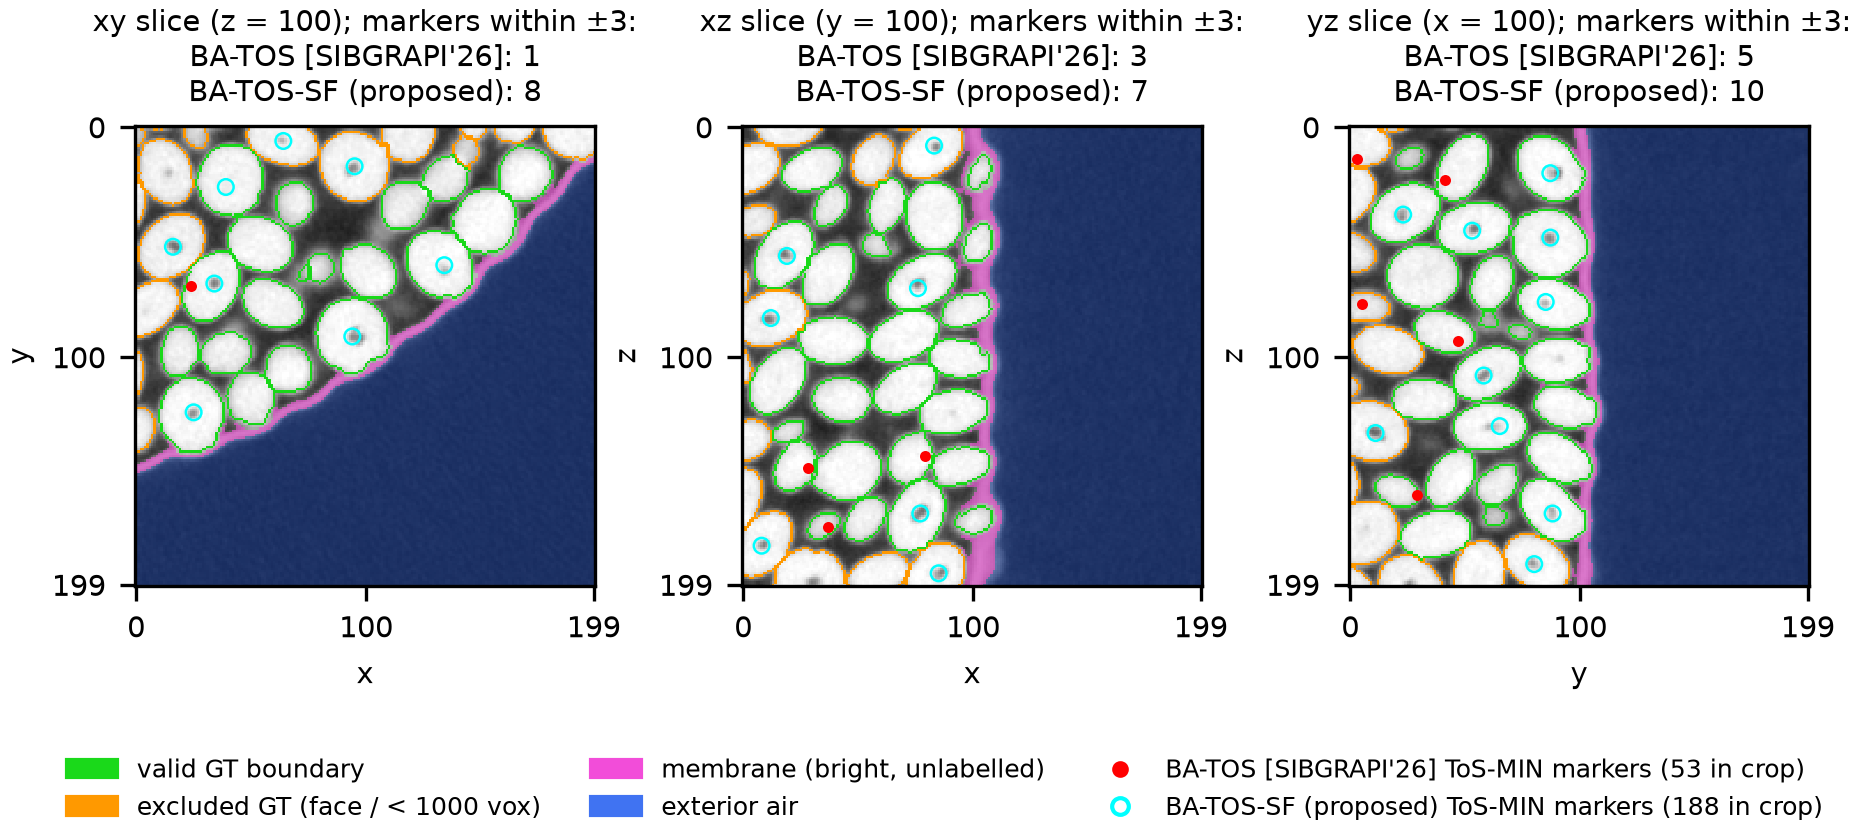
\includegraphics[width=0.88\textwidth]{fig2_crop05_orthogonal_markers.png}
\caption{EFRGP01\_00\_crop05, central orthogonal slices. Green: valid GT boundaries; orange: excluded GT; magenta:
confining membrane; blue: exterior air (51\,\% of the crop). Red dots: the 53 ToS-MIN markers of \SIB, in pores and
air; cyan rings: the 188 markers of \SF, about one per grain. Membrane and air are display masks only.}
\label{fig:crop05}
\vspace{4pt}
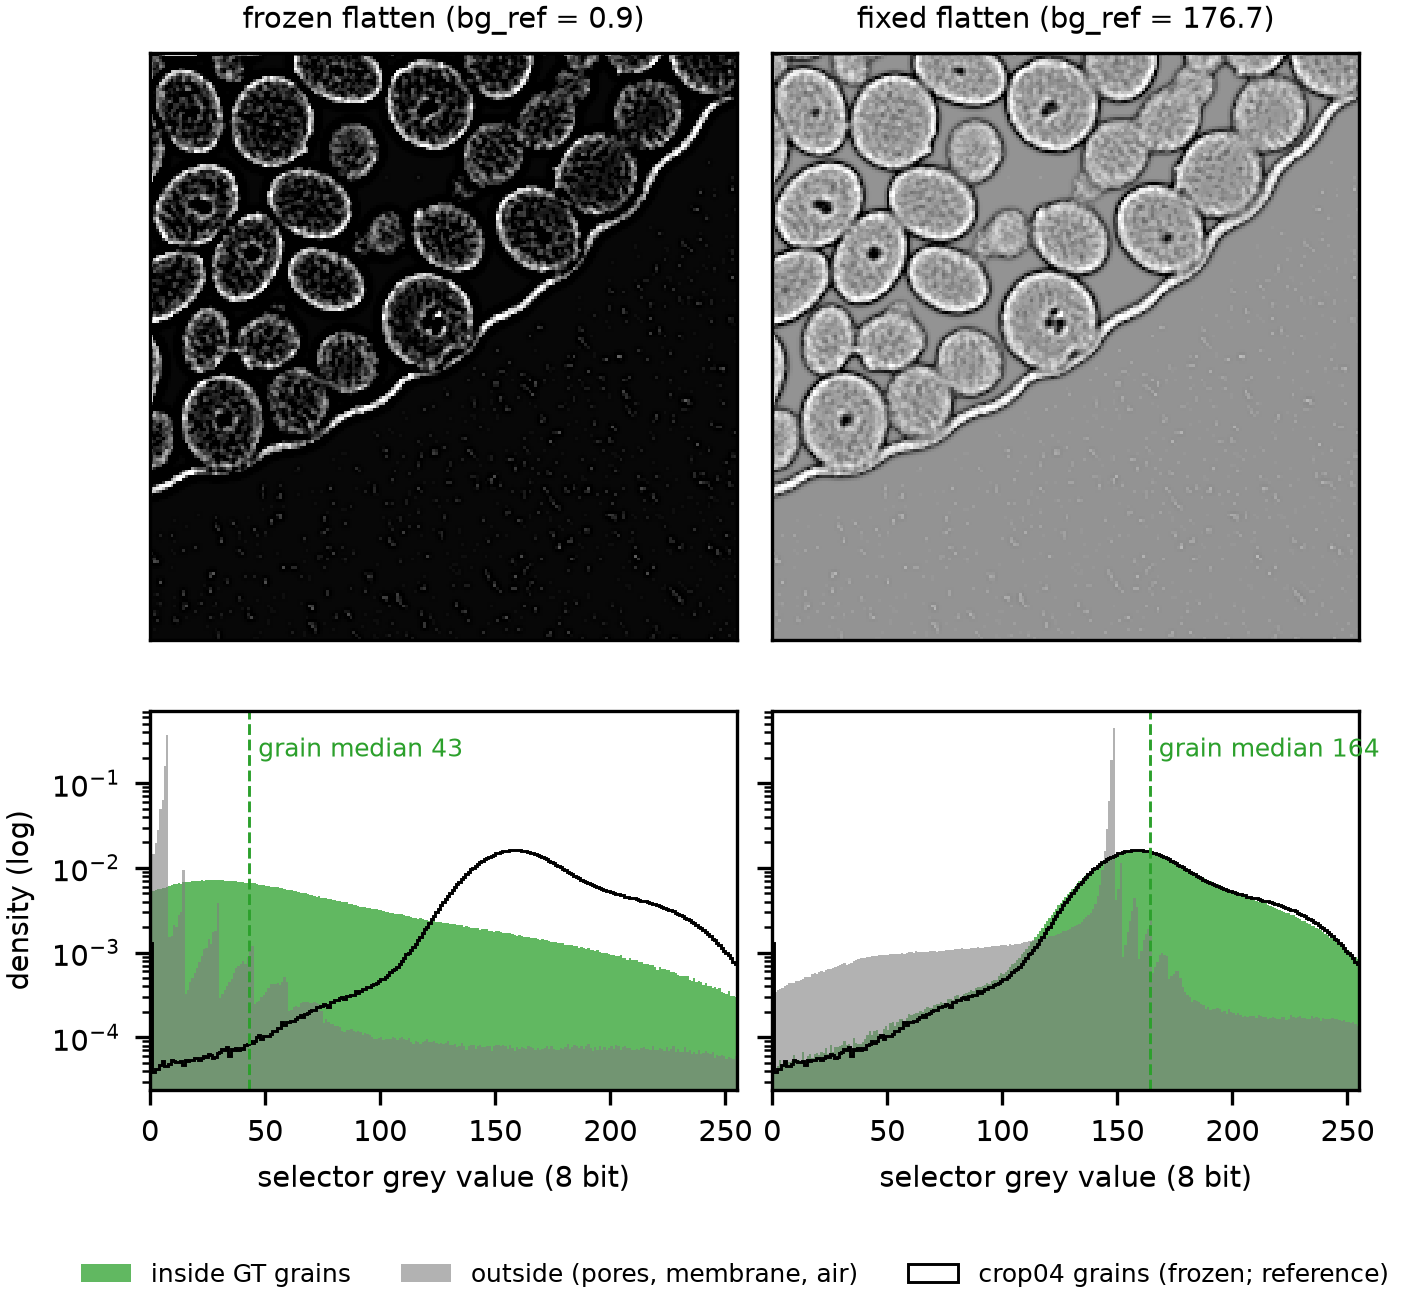
\includegraphics[width=0.62\textwidth]{fig3_crop05_flatten_offset.png}
\caption{Selector flatten on EFRGP01\_00\_crop05 with intensity histograms (green: GT grain voxels; grey: others;
black outline: crop04 grains for reference). Left, \SIB: the offset falls to 0.9 and grains lose their contrast
(grain median 43). Right, specimen-only offset (176.7): the grain histogram returns to the crop04 reference.}
\label{fig:offset}
\end{figure}

\textbf{The scale estimator on larger grains.} BA-TOS derives its opening radius from a GT-free scale estimate
$\hat r$, the median of the 1,500 highest local maxima of the Euclidean distance transform (EDT) of the Otsu
foreground. On the development crops it is approximately right, but it is biased by the composition of the crop and
it halves the radius on the larger grains of the EM and EO specimens (Fig.~\ref{fig:scale}, right): only 19 of 63
crops are within $\pm$10\,\% of the GT median inscribed radius (median relative error $-$25\,\%). Since the opening
radius is the most influential constant of the pipeline (Section~\ref{sec:audit}), this error propagates to the
whole chain. In addition, the published code contains absolute constants (sizes in voxels, grey-level thresholds)
calibrated for EFR grains of radius $\approx$10 voxels.

\begin{figure}[t]
\centering
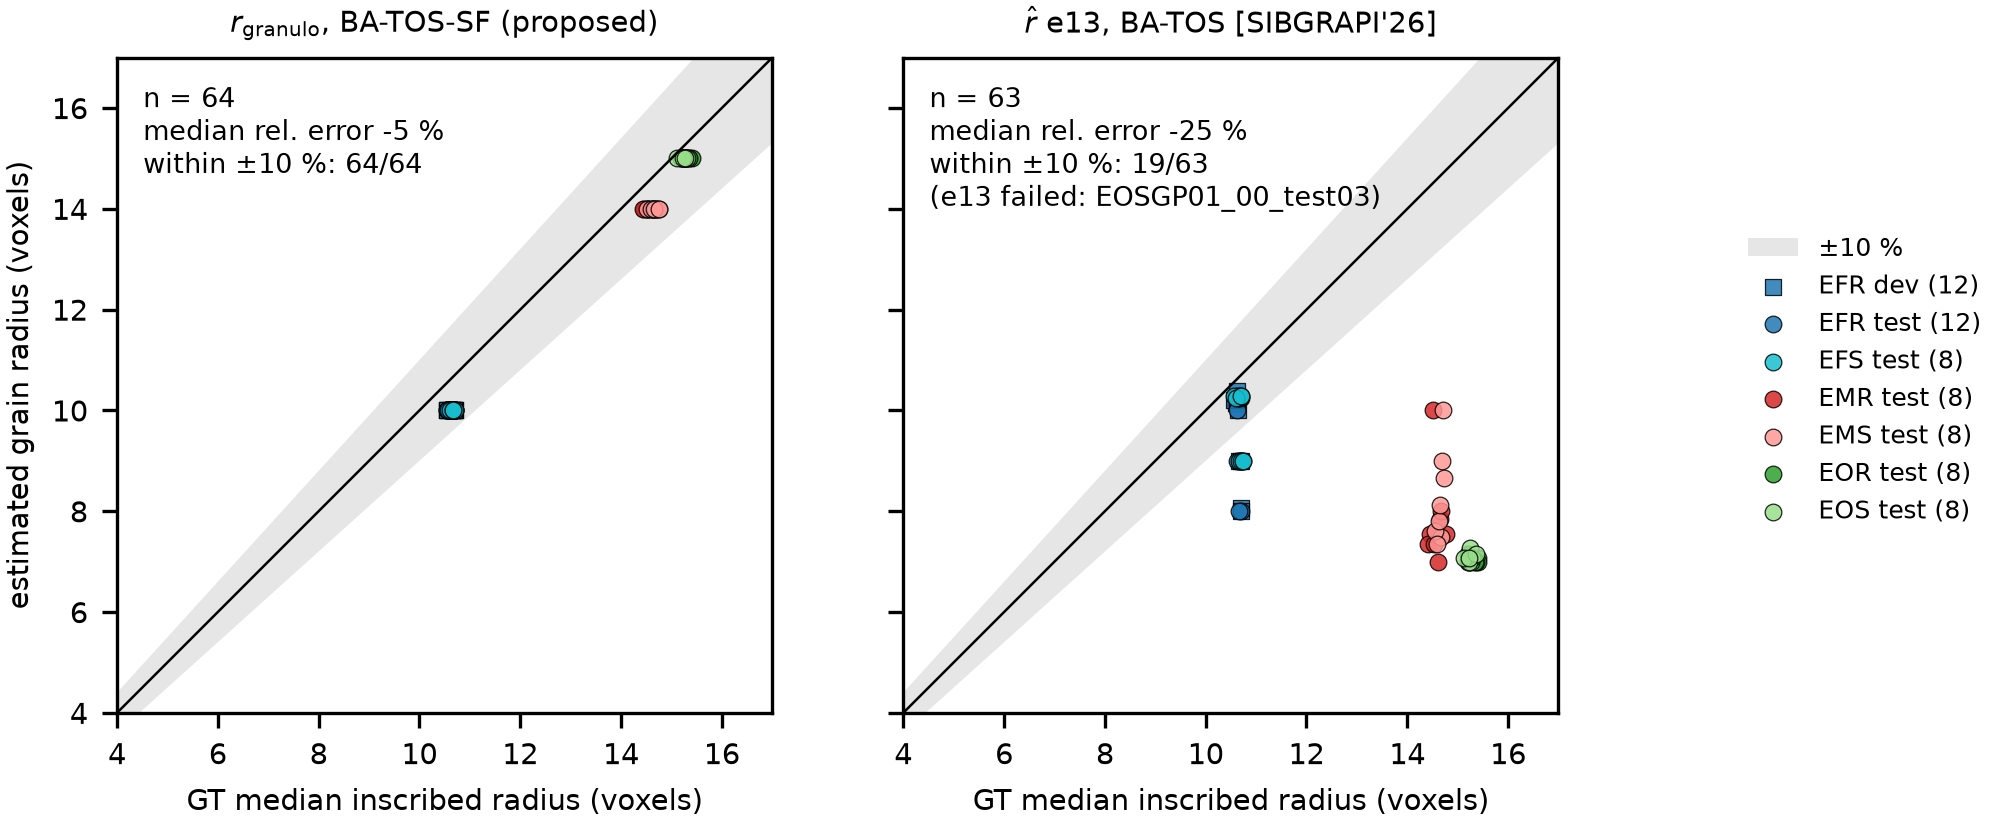
\includegraphics[width=0.80\textwidth]{fig4_scale_estimates.png}
\caption{GT-free grain-radius estimates against the GT median inscribed radius for 64 crops (12 development, squares;
52 test, circles), coloured by specimen. Left, $\rg$ of \SF: 64/64 within $\pm$10\,\% (median error $-$5\,\%).
Right, $\hat r$ of \SIB: 19/63 within $\pm$10\,\% (median $-$25\,\%; the estimator failed on one crop). The GT
radius is used for diagnosis only.}
\label{fig:scale}
\end{figure}

\subsection{BA-TOS-SF: a scale-free pipeline}
\label{sec:sf}

\SF{} keeps the structure of BA-TOS (ToS-MIN candidates, boundary rejection, internal markers, safeguard, watershed)
and changes where its constants come from.

\textbf{Granulometric scale.} The grain radius $\rg$ is the mode of the pattern spectrum \citep{maragos1989} of the
specimen foreground: binary openings by exact Euclidean balls of radius $r = 2,\ldots,40$ (computed with EDTs) and
$\rg = \arg\max_r \mathrm{PS}(r)$, with $\mathrm{PS}(r) = V(r) - V(r{+}1)$. The foreground is estimated in two passes:
a first Otsu foreground (with holes filled) gives $r_0$; the specimen is the largest component of its closing by a
ball of radius $2r_0$; Otsu is then recomputed on specimen voxels only. The estimator has no free parameter; on all
12 development crops it returns $\rg = 10$ (GT inscribed radius 10.6), and on all 64 crops it is within
$\pm$10\,\% of the GT radius (Fig.~\ref{fig:scale}, left).

\textbf{Scaled constants.} With $s = \rg/10$, every constant is classified by its physical dimension and scaled
accordingly: lengths by $s$, volumes and ToS areas by $s^3$, object counts per crop (such as the candidate
capacity $K$) by $1/s^3$; dimensionless constants (weights, ratios, percentiles, $\tau_s = 0.35$) are kept. On the
development crops $s=1$, so every scaled constant equals its published value.

\textbf{Specimen-only statistics and removed guards.} Thresholds that mixed a statistic with ad-hoc corrections are
replaced by the same statistic computed on specimen voxels, and absolute grey-level guards that never or almost never
acted are removed (Table~\ref{tab:constants}). The safeguard limits are scaled as $3\max(1,s^3)$ and $4\max(1,s^3)$,
since a collapsed support is a discretization degeneracy of 1--3 voxels.

\begin{table}[t]
\centering
\caption{Constants of the published pipeline (93, as inventoried in the code) and their treatment in \SF, with the
main replaced rules.}
\label{tab:constants}
\small
\begin{tabular}{p{5.0cm}cc}
\toprule
Constants & \SIB & \SF \\
\midrule
Fixed in voxels (lengths, volumes, counts) & 43 & 0 (scaled by $s$, $s^3$, $1/s^3$) \\
Ad-hoc thresholds and rules & 6 & 0 (replaced by rules) \\
Absolute grey-level guards & 3 & 0 (removed) \\
Dimensionless (weights, ratios, percentiles) & 41 & 41 (kept) \\
\midrule
Scale source & EDT maxima ($\hat r$) & pattern spectrum ($\rg$) \\
Flatten offset & median$(\mathit{blur} > 0)$ & median$(\mathit{blur} \ge 1)$ \\
Dark threshold & $\min(\mathrm{Otsu}-10,\ p_{40},\ 135)$ & Otsu on specimen \\
Safeguard limits $m_v$, $q_v$ & 3, 4 & $3\max(1,s^3)$, $4\max(1,s^3)$ \\
\bottomrule
\end{tabular}
\end{table}

\textbf{Design discipline.} \SF{} was designed on the 12 development crops and on a synthetic scale set (the
development crops rescaled by factors 0.7, 1.4 and 2.0, i.e.\ 36 additional crops), then frozen (version tag and
SHA-256 of all executed code) before the held-out crops were read.

\subsection{Parameter audit}
\label{sec:audit}

To measure which constants matter, the 96 method constants of the published pipeline (selector, opening and
flattening, markers, safeguard and watershed) were perturbed one at a time, typically to half and double their
value, on all 12 development crops (2,242 completed crop runs). The effect of a constant is the largest absolute change
in crop-macro F1@0.50; a constant is called influential if the effect exceeds 0.01.

\subsection{Foundation-model baseline}

\CP{} is run with one fixed configuration per model and no fine-tuning or per-crop tuning: 3D mode, Cellpose's own
scale (no rescaling), default flow smoothing, on a single 8\,GB GPU. The default \texttt{cpsam\_v2} is the main
baseline; the other three Cellpose~4 models were also evaluated. Since Cellpose produces no seeds, it is evaluated
in the no-marker mode, and \SF{} is reported in the same mode for the comparison. A small sensitivity check (flow
smoothing 1 and 2, diameter set from $\rg$) was run on the development crops only. We checked the training data of
Cellpose-SAM against the preprint \citep{pachitariu2025}: the documented set is 2D cells and nuclei (plus 98
natural photographs inherited from the original Cellpose dataset), with no micro-CT, granular material or Zenodo
8014905 data. The training sets of the June 2026 models are not documented, but the documented \texttt{cpsam}
gives the same results. Robustness was tested on three crops with additive Gaussian noise (2, 5 and 10\,\% of the
grain--air contrast) and $2\times$ downsampling, and on the synthetic scale set.

% ---------------------------------------------------------------------------
\section{Preliminary Results}

\subsection{Development crops}

Table~\ref{tab:dev} summarizes the development results. The offset correction alone raises the crop-macro F1@0.50 of
the ToS route from 0.824 to 0.976 and makes the safeguard unnecessary; \SF{} reaches 0.989 with a minimum of 0.974.
On the synthetic scale set, \FIX{} collapses when grains are larger (0.750 at $1.4\times$, 0.239 at $2\times$),
whereas \SF{} holds (0.975 / 0.995 / 0.938 at $0.7$ / $1.4$ / $2.0\times$; 1.000 at $1.4$ and $2\times$ with its
scaled size filter).

\begin{table}[t]
\centering
\caption{Development crops (12 EFR crops): F1@0.50, seed-ignore, no size filter. Crop-macro: mean $\pm$ SD (min).}
\label{tab:dev}
\small
\begin{tabular}{lcc}
\toprule
Method & Crop-macro F1@0.50 & Pooled F1@0.50 \\
\midrule
\SIB, without safeguard & $0.824 \pm 0.367$ (0.012) & 0.912 \\
\SIB, with safeguard & $0.906 \pm 0.210$ (0.260) & 0.950 \\
\FIX & $0.976 \pm 0.023$ (0.913) & 0.979 \\
\SF{} (proposed) & $\mathbf{0.989 \pm 0.008}$ (0.974) & \textbf{0.988} \\
\bottomrule
\end{tabular}
\end{table}

\subsection{Held-out test set}

Table~\ref{tab:test} gives the results on the 52 held-out crops. \SF{} raises the crop-macro F1@0.50 from 0.538
(\SIB) and 0.575 (\FIX) to 0.912, and the pooled F1@0.50 from 0.700 and 0.752 to 0.921. It never crashes (the other
two methods crash on 1 and 5 crops) and its safeguard never fires (30 and 13 activations). On the EF and EM
specimens it reaches 0.974--0.986, while the published method nearly fails on EM (0.303 and 0.432) because of its
scale estimate. The offset correction helps on EF but not on EM and EO, where the scale is the limiting factor. On
the large-grained EO specimens \SF{} reaches only 0.754 (Section~\ref{sec:eo}). Figure~\ref{fig:slices}
illustrates these behaviours: the published method merges the EMR crop into a single label, and \SF{} under-seeds
the larger EO grains.

\begin{table}[t]
\centering
\caption{Held-out test set (52 crops of $200^3$, 6 specimens): crop-macro F1@0.50 (mean $\pm$ SD) and pooled
F1@0.50, seed-ignore, no size filter. $\rg$ / $r_{\mathrm{in}}$: \SF{} scale estimate / GT median inscribed radius
(diagnostic only).}
\label{tab:test}
\setlength{\tabcolsep}{3pt}
\resizebox{\textwidth}{!}{%
\begin{tabular}{lrccccccc}
\toprule
 & & & \multicolumn{3}{c}{Crop-macro F1@0.50} & \multicolumn{3}{c}{Pooled F1@0.50} \\
\cmidrule(lr){4-6}\cmidrule(lr){7-9}
Specimen & $n$ & $\rg$ / $r_{\mathrm{in}}$ & \SIB & + corr.\ flat. & \SF & \SIB & + corr.\ flat. & \SF \\
\midrule
EFR & 12 & 10 / 10.6 & $0.879 \pm 0.223$ & $0.956 \pm 0.048$ & $\mathbf{0.985 \pm 0.011}$ & 0.929 & 0.967 & \textbf{0.985} \\
EFS &  8 & 10 / 10.6 & $0.882 \pm 0.155$ & $0.968 \pm 0.043$ & $\mathbf{0.974 \pm 0.044}$ & 0.881 & 0.965 & \textbf{0.970} \\
EMR &  8 & 14 / 14.5 & $0.303 \pm 0.439$ & $0.250 \pm 0.416$ & $\mathbf{0.980 \pm 0.027}$ & 0.393 & 0.371 & \textbf{0.973} \\
EMS &  8 & 14 / 14.7 & $0.432 \pm 0.465$ & $0.479 \pm 0.474$ & $\mathbf{0.986 \pm 0.020}$ & 0.495 & 0.546 & \textbf{0.983} \\
EOR &  8 & 15 / 15.3 & $0.293 \pm 0.362$ & $0.238 \pm 0.434$ & $\mathbf{0.754 \pm 0.240}$ & 0.350 & 0.324 & \textbf{0.733} \\
EOS &  8 & 15 / 15.3 & $0.265 \pm 0.429$ & $0.365 \pm 0.499$ & $\mathbf{0.754 \pm 0.214}$ & 0.311 & 0.455 & \textbf{0.735} \\
\midrule
External (5 spec.) & 40 & -- & $0.435 \pm 0.435$ & $0.460 \pm 0.473$ & $\mathbf{0.890 \pm 0.178}$ & 0.585 & 0.635 & \textbf{0.893} \\
All & 52 & -- & $0.538 \pm 0.437$ & $0.575 \pm 0.465$ & $\mathbf{0.912 \pm 0.161}$ & 0.700 & 0.752 & \textbf{0.921} \\
\midrule
\multicolumn{3}{l}{Crops with F1 $<0.90$} & 33 & 25 & \textbf{10} & & & \\
\multicolumn{3}{l}{Crashes (scored empty)} & 1 & 5 & \textbf{0} & & & \\
\multicolumn{3}{l}{Safeguard fires} & 30 & 13 & \textbf{0} & & & \\
\bottomrule
\end{tabular}}
\end{table}

\subsection{Sensitivity of the published constants}

All 96 constants have a complete ranking; 25 are influential (effect $>0.01$) and 71 are not. The most influential
are the opening radius factor (effect 0.883; factor 0.75 collapses every crop), the flattening $\lambda$ (0.637), and
the selector's area prior and weights: \texttt{area\_preferred\_position} (0.613), \texttt{w\_delta} (0.512),
\texttt{w\_area} and \texttt{area\_preferred\_width} (0.417 each), followed by the minimum ToS area (0.289), the
absolute dark threshold cap of 135 (0.229), the height-scale percentile (0.216) and the candidate capacity $K$
(0.127). The selector weights sit on a narrow ridge: halving or doubling one of them drops F1 by 0.4--0.6, and one
weight (\texttt{w\_support}) has no effect at all. The two most influential constants are exactly the scale-dependent
ones that \SF{} now derives from $\rg$, and the dark-threshold cap is one of the absolute guards it removes.

\subsection{Comparison with Cellpose-SAM}
\label{sec:cellpose}

Table~\ref{tab:cellpose} compares \SF{} with \CP{} under the no-marker evaluation. \CP{} reaches 0.998 crop-macro
F1@0.50 on both splits and is above 0.98 on every specimen; no crop is below 0.90 (10 for \SF). The four Cellpose~4
models agree within 0.002, the development sensitivity check leaves the score unchanged (0.997--0.999), and the
documented model gives the same result, so the result is not an artefact of one checkpoint, one setting, or data
leakage. The gap is concentrated on EO (0.996--0.998 vs 0.727--0.735).

\begin{table}[t]
\centering
\caption{\CP{} (\texttt{cpsam\_v2}, default settings) vs \SF: crop-macro F1@0.50, no-marker evaluation, no size
filter. mIoU: mean IoU of matched grains (test).}
\label{tab:cellpose}
\small
\begin{tabular}{lccc}
\toprule
Scope & $n$ & \CP & \SF \\
\midrule
Development (EFR) & 12 & \textbf{0.998} & 0.979 \\
Test EFR / EFS & 12 / 8 & \textbf{0.999} / \textbf{0.999} & 0.977 / 0.964 \\
Test EMR / EMS & 8 / 8 & \textbf{0.998} / \textbf{0.999} & 0.966 / 0.970 \\
Test EOR / EOS & 8 / 8 & \textbf{0.996} / \textbf{0.998} & 0.735 / 0.727 \\
Test, all & 52 & $\mathbf{0.998 \pm 0.004}$ & $0.896 \pm 0.168$ \\
Test pooled (TP / FP / FN) & 8,614 & \textbf{0.998} (8613 / 32 / 1) & 0.907 (7437 / 354 / 1177) \\
Test mIoU@0.50 & & 0.899 & \textbf{0.902} \\
\bottomrule
\end{tabular}
\end{table}

\textbf{Robustness.} Table~\ref{tab:robust} shows that \CP{} is essentially insensitive to added noise and
downsampling, whereas \SF{} collapses at 5\,\% noise on all three crops: noise multiplies small dark extrema, which
saturate the ToS candidate capacity (surviving ToS markers on crop04: 396, 374, 78, 5 from clean to 10\,\%). On
the synthetic scale set \CP{} scores 1.000 / 0.999 / 0.963 at $0.7$ / $1.4$ / $2.0\times$ and \SF{} 0.972 / 0.979
/ 0.900 (no-marker mode). Since Cellpose-SAM was trained with noise, blur, downsampling and rescaling augmentations,
these are expected behaviours rather than luck.

\begin{table}[t]
\centering
\caption{Robustness, F1@0.50 (no-marker mode). Noise: additive Gaussian, $\sigma$ in \% of the grain--air contrast;
$0.5\times$: $2\times2\times2$ block-mean downsampling, predictions upsampled and scored on the original GT.}
\label{tab:robust}
\small
\begin{tabular}{llccccc}
\toprule
Crop & Method & clean & 2\,\% & 5\,\% & 10\,\% & $0.5\times$ \\
\midrule
\multirow{2}{*}{EFRGP01\_00\_crop04} & \CP & 1.000 & 1.000 & 1.000 & 1.000 & 1.000 \\
 & \SF & 0.980 & 0.912 & 0.127 & 0.000 & 0.662 \\
\multirow{2}{*}{EORGP01\_00\_test01} & \CP & 0.980 & 0.980 & 0.977 & 0.977 & 0.985 \\
 & \SF & 0.544 & 0.685 & 0.062 & 0.000 & 0.979 \\
\multirow{2}{*}{EORGP01\_00\_test04} & \CP & 1.000 & 1.000 & 1.000 & 0.990 & 1.000 \\
 & \SF & 0.985 & 0.941 & 0.000 & 0.000 & 0.976 \\
\bottomrule
\end{tabular}
\end{table}

\textbf{Boundaries.} On grains matched by both methods, \CP{} has a systematic $\approx$1-voxel outward bias: its
contours sit about one voxel outside the GT (Fig.~\ref{fig:boundary}a,b), with a median volume error of $+11.7\,\%$
on crop04 and $+9.4\,\%$ on EORGP01\_00\_test01, in a narrow band. \SF{} is centred nearer zero on crop04 (median
$-3.7\,\%$, IQR $-4.1$ to $+5.3\,\%$) and $+6.4\,\%$ on the EO crop, and its matched IoU on the test set is
slightly higher (0.902 vs 0.899). This advantage must be stated with its caveat: \SF{} has a heavy over-volume tail
(46 of 259 grains above $+20\,\%$ on crop04, 28 of 69 on the EO crop, maximum $+91\,\%$), so its \emph{mean} shape
errors (sphericity, Hausdorff distance) are worse than those of \CP. Moreover, a 1-voxel erosion of the Cellpose
masks raises its test mIoU to 0.917, and the DINOv3-based Cellpose model already reaches 0.928.

\begin{figure}[t]
\centering
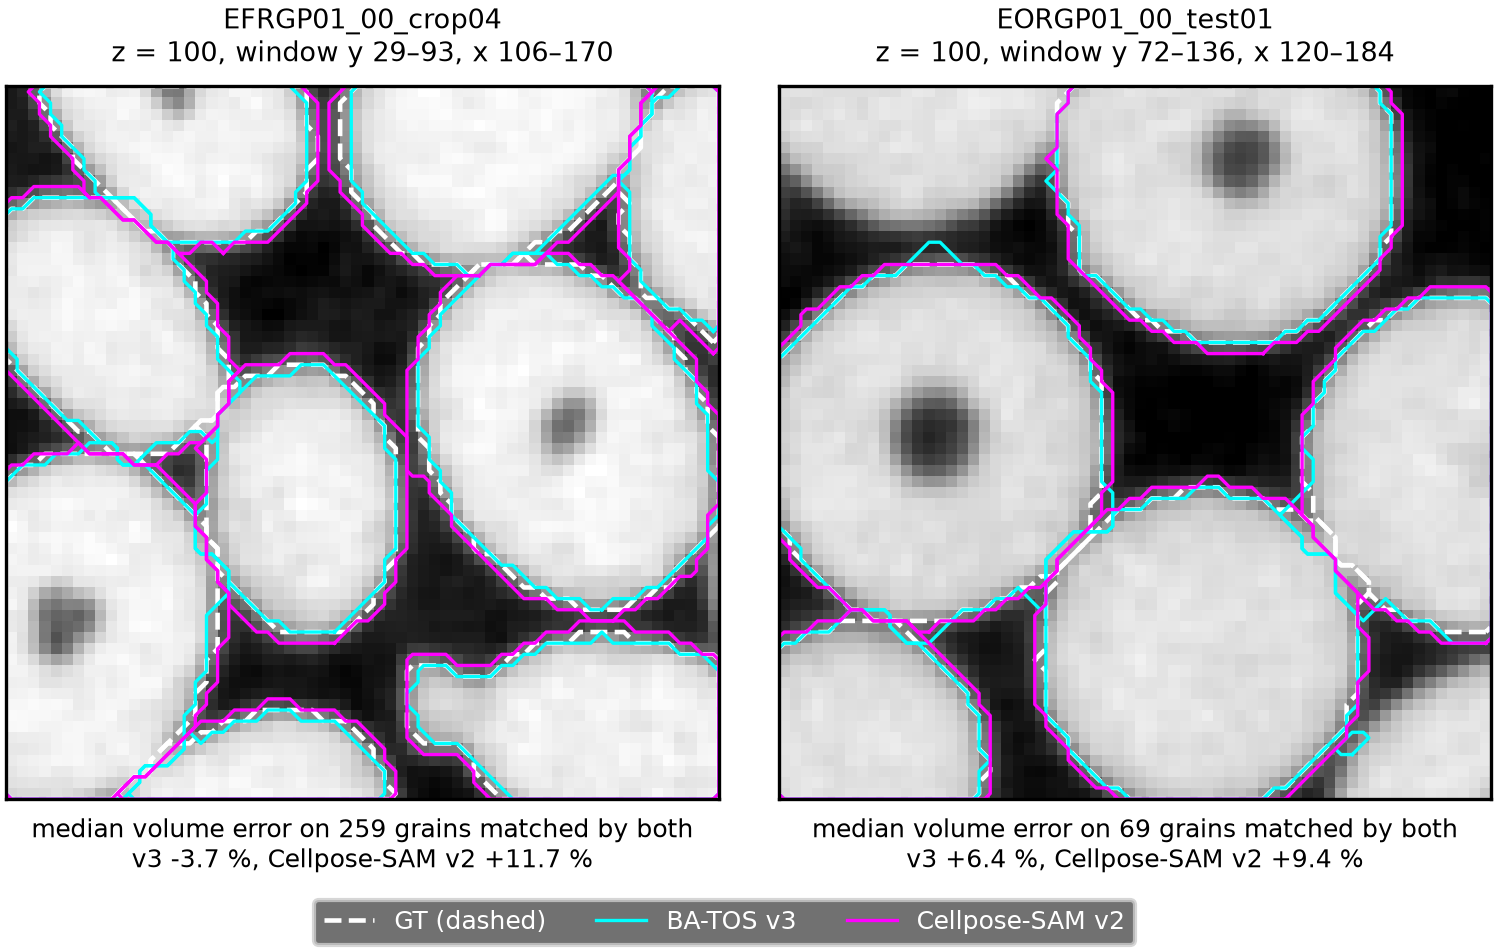
\includegraphics[width=0.85\textwidth]{fig5_boundary_contours.png}
\caption{Boundary fidelity on grains matched (IoU $>0.5$) by both methods. (a, b) Contours on $32\times32$ windows of
crop04 and EORGP01\_00\_test01 (white dashed: GT; cyan: \SF; magenta: \CP). (c) Per-grain relative volume error;
solid: crop04 (259 grains), dashed: EOR test01 (69 grains); vertical lines: medians; values above $+60\,\%$ (18
grains, all \SF) are drawn in the last bin.}
\label{fig:boundary}
\end{figure}

\subsection{The EO limitation: candidate capacity}
\label{sec:eo}

The low EO scores are not a scale-estimation error ($\rg = 15$ for $r_{\mathrm{in}} = 15.3$). They come from the
candidate capacity: the number of ToS-MIN candidates is capped at $1800/s^3$, i.e.\ 533 at $s = 1.5$, and the cap is
reached on every test crop. On the interior EO crops, which hold about 168 valid grains, this leaves 1.2 candidates
per grain and 0.35 ToS markers per grain (about 0.6 on all other specimens and on EO boundary crops), so roughly a
third of the grains receive no marker and are merged with a neighbour or missed. The median F1@0.50 is 0.556 / 0.548 on
interior EOR / EOS crops, against 0.978 / 0.983 on their boundary crops. Two observations confirm the mechanism:
downsampling EORGP01\_00\_test01 by 2 brings its grains back under the cap and its F1 from 0.544 to 0.979
(Table~\ref{tab:robust}), and noise, which saturates the cap with spurious extrema, produces the same collapse.
Raising the capacity alone is not sufficient: a variant that floors the counts at their published values increases
the markers per grain but over-segments into small fragments, so the capacity must be coupled to a rule that keeps
one marker per grain.

% ---------------------------------------------------------------------------
\section{Next Steps until TCC II}

\textbf{Full-volume tiled segmentation.} The method was frozen on $200^3$ crops; applying it to a full scan
(EFRGP01\_00 is $1600\times1400\times1400$ voxels) requires tiling. The design, fixed GT-free before any run, uses
cores of $160^3$ with a halo of $\lceil 2\rg\rceil = 20$ voxels, i.e.\ padded tiles of exactly $200^3$, the volume the
method was designed on; one scale per scan ($\rg$ of the central crop); only tiles whose core touches the specimen
(277 of 810); ownership of an instance by the tile containing its centroid; and stitching by one-to-one IoU
$\ge 0.5$ matching with an orphan-rescue step for seam grains owned by no tile. A smoke test on the central
$3\times3\times3$ tiles (cores of $200^3$, $600^3$ in total) produced 9,753 instances and F1@0.50 = 0.865 on the
6,005 valid GT grains (seed-ignore; 0.827 without orphan rescue). It also showed why the $160^3$ cores are needed:
with larger tiles the fixed candidate pool is diluted and interior recall drops. The full run will be evaluated on
the authors' region of interest of the scan.

\textbf{Grain tracking.} The dataset includes the authors' tracking files between consecutive scans (e.g.\
\texttt{EFRGP01\_00\_01}). We will match \SF{} instances between scans \texttt{00} and \texttt{01} and compare the
resulting correspondences and displacements with the authors' tracking, which tests the segmentation on a
downstream task rather than on overlap alone. Contact recall against the authors' contact lists, already computed
on the 64 crops (0.782 for \SF, 1.000 for \CP), will be extended to the full volume.

\textbf{Morphological descriptors.} Volume, equivalent diameter, surface area, sphericity, elongation, orientation
and centroid error will be computed per grain and compared with the GT, separating the systematic bias of each
method (such as the 1-voxel dilation of \CP) from its tail of badly shaped grains. The EO capacity limit will be
addressed by a capacity rule coupled with per-grain uniqueness, designed on the development and synthetic crops and
frozen before a second held-out set is cut.

\textbf{Writing.} The results will be consolidated into the TCC~II text and a journal extension of the SIBGRAPI
paper. Given Table~\ref{tab:cellpose}, the journal framing is a benchmark and protocol contribution: a pre-registered
64-crop, six-specimen benchmark; the effect of evaluation rules (face exclusion and ignore rules) on rankings;
and \SF{} as a transparent, training-free reference whose failure modes are explained, alongside Cellpose-SAM as
the learned reference.

\bibliographystyle{apalike}
\bibliography{references}

\end{document}
